\chapter{System Overview}

In order to understand the process of the recovery of rare earth elements from electronic waste with biosorption, the key procedures and techniques are described briefly in the following section.

\section{Detection of REEs\authorA}

A relatively simple proof if a probe contains REEs is a precipitation reaction.
It works by utilizing the +III and the +IV oxidization states of the REEs.
These are used to form complexes with other molecules which express themselves as a coloured precipitation in the probe solution \footnote{Jander/Blasius: "Lehrbuch der analytischen und präparativen anorganischen Chemie", Chapter 4.3.3.10}.
As an example, a Ce precipitation reaction is shown in~\ref{fig:cer_precipitation_cropped} with an orange-red precipitate.

\begin{figure}[H]
    \centering
    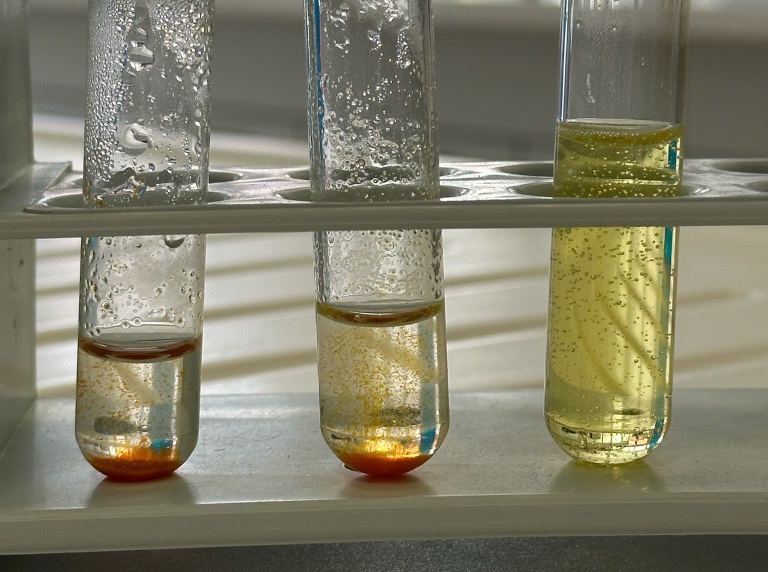
\includegraphics[width=0.75\textwidth]{./media/images/ree_precipitation_reaction_cropped}
    \caption{Precipitations of a successful REE detection reaction. The test tube on the righthandside does not show any precipitation because the probe was deionized water.}
    \label{fig:cer_precipitation_cropped}
\end{figure}

However, you must be careful, because of the REEs chemical similarity, the detection of a specific REE is not always possible with these precipitation methods.


\section{Bacteria}

Lorem ipsum dolor sit amet, consectetur adipiscing elit. Aenean viverra eget sapien in fringilla. Proin ac neque non lectus vehicula laoreet in cursus enim. Donec et erat ut erat commodo viverra vitae sed risus. Etiam tortor justo, placerat in turpis sit amet, egestas tristique libero. Phasellus metus arcu, viverra at interdum ac, convallis non urna. Sed nunc libero, elementum quis ultricies at, vestibulum in arcu. Nam ultrices felis ut sagittis hendrerit. Vivamus massa sapien, interdum nec dui ac, consectetur venenatis dolor. Integer enim felis, finibus at efficitur eget, viverra vitae purus. Curabitur at libero pretium, vestibulum lacus at, eleifend nisl.

\subsection{Methylorubrum extorquens}

\subsection{Cultivation}

\section{Lanmodulin\authorA}

Lanmodulin (LanM) is a protein that is produced by \textit{M. extorquens}, a lanthanide-utilizing bacteria~\cite{lanmdiscovery}.
LanM is not essential for the growth or survival of \textit{M. extorquens}, and it is only produced when the bacteria are in a medium with presence of \ce{Ln^{III}} or \ce{Ce^{III}} ions~\cite{lanmroleinbiology}.
However, the mechanisms that include LanM are not understood as a whole to this day.

\begin{figure}[H]
    \centering
    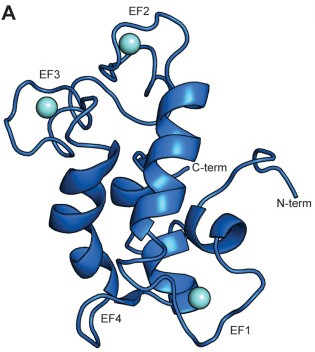
\includegraphics[width=0.6\textwidth]{./media/images/lanm_structure}
    \caption{Graphical visualisation of the structure of lanmodulin. The EF-hands are indicated by EF, this is where the REEs can bind to the protein. In this visualisation the turquoise coloured spheres are \ce{Y^{III}} ions which are bound to the EF-hands. Picture from "The biochemistry of lanthanide acquisition, trafficking and utilization", Emily R. Featherston and Joseph A. Cotruvo \cite{lanmroleinbiology}.}
    \label{fig:lanm_structure}
\end{figure}

The most important characteristic of LanM is, that the molecule is able to bind lanthanide ions, primarily light REEs (LREEs).
When LanM does this, it undergoes a transformation from a disordered state to a compact form of itself.
The REEs are hereby bound to the so-called EF-hands which favour to bind to \ce{Ln^{III}} and other lanthanoids over \ce{Ca^{II}} which is usually associated with these EF-hands~\cite{lanmstructure}.


\section{Protein Extraction}

\subsection{Cell Lysis}

\subsection{SDS-PAGE}

\section{IR-Spectrometry}